\documentclass[a4paper,12pt]{article}

% Packages
\usepackage[T1]{fontenc}
\usepackage{lmodern}
\usepackage[utf8]{inputenc}
\usepackage{graphicx}  % For images
\usepackage{listings}  % For code snippets
\usepackage{xcolor}    % For code coloring
\usepackage{hyperref}  % For hyperlinks
\usepackage{amsmath}   % For math equations
\usepackage{caption}   % Better captions
\usepackage{geometry}  % Page layout
\geometry{margin=2.5cm}
\usepackage{graphicx}
\usepackage{subcaption}
\usepackage{listings}
\usepackage{float}  % Optional, for better figure placement


% Remove paragraph indentation
\setlength{\parindent}{0pt}

% Code styling
\lstset{
    language=Python,
    basicstyle=\ttfamily\footnotesize,
    keywordstyle=\color{blue},
    stringstyle=\color{red},
    commentstyle=\color{gray},
    breaklines=true,
    frame=single
}

\title{Lab Report: \textbf{Motion Recognition using IMU Sensor Fusion}}
\author{Student Name: Charanjit Bangalore Kumar \\ Student ID: 12504134 \\ Course Name: Embedded System \\ Instructor: Prof. Tobias Schaffer}
\date{Date: 11/06/2025}

\begin{document}

\maketitle

\section{Introduction}
This lab focuses on recognizing human motion using Inertial Measurement Unit (IMU) data from a Raspberry Pi Sense HAT. The goal is to capture sensor data, train a neural network to classify motion patterns, and deploy the trained model to perform real-time gesture recognition and respond by lighting LEDs accordingly.
\section{Objectives}
The main objectives of this lab are:
\begin{itemize}
    \item Collect motion data using the Raspberry Pi Sense HAT (accelerometer + gyroscope).
    \item Label four motion types: \texttt{move\_none}, \texttt{move\_circle}, \texttt{move\_shake}, \texttt{move\_twist}.
    \item Train a neural network model using TensorFlow in Google Colab.
    \item Convert the trained model to TensorFlow Lite format.
    \item Deploy and run the model on Raspberry Pi to recognize gestures in real time.
    \item Display the LED matrix based on predicted gestures.
\end{itemize}


\section{Methodology}
This project follows a pipeline that includes data collection, pre-processing, model training, and deployment. IMU data are captured from the Raspberry Pi's Sense HAT for different gestures. This labeled sensor data is then used to train a neural network using TensorFlow. Once trained, the model is converted to TensorFlow Lite and deployed back onto the Raspberry Pi for real-time inference and LED-based gesture feedback.

\subsection{Data Collection}

Motion data was collected using the Raspberry Pi Sense HAT's IMU sensors (accelerometer + gyroscope). For each gesture, 50 samples were collected at a sampling rate of \textbf{50 Hz}, giving \textbf{1.0 second} of data per gesture instance. Each sample contains six features: three-axis accelerometer values and three-axis gyroscope values.

\begin{itemize}
 \item Sensors: 3-axis accelerometer and 3-axis gyroscope
 \item Sampling rate: 50 Hz
 \item Samples per gesture: 50
 \item Total features per gesture: $50 \times 6 = 300$
 \item Data format: \texttt{[acc\_x, acc\_y, acc\_z, gyro\_x, gyro\_y, gyro\_z]}
\end{itemize}

% \subsection{Data Preprocessing}

% The raw sensor data is flattened into one-dimensional arrays suitable for input to a dense neural network. Each gesture sample becomes a vector of 1800 features (300 time steps $\times$ 6 features). The corresponding gesture labels are encoded using one-hot encoding. Optional preprocessing steps such as normalization or filtering may also be applied to improve learning.

% \begin{itemize}
%     \item Flattened feature vector: \texttt{300 $\times$ 6 = 1800}
%     \item Labels: One-hot encoded for four gesture classes
%     \item Goal: Ensure input data is in a suitable and consistent format for training
% \end{itemize}

\subsection{Model Training}

Model training is conducted using TensorFlow in Google Colab. The architecture consists of a feedforward neural network with two hidden layers and dropout for regularization.

\begin{itemize}
    \item Input layer: 1800 neurons
    \item Hidden layers:
    \begin{itemize}
        \item Dense(128, ReLU)
        \item Dropout(0.2)
        \item Dense(64, ReLU)
    \end{itemize}
    \item Output layer: Dense(4, Softmax) for classifying the four gestures
    \item Optimizer: Adam
    \item Loss function: Categorical crossentropy
    \item Epochs: 15
    \item Batch size: 32
\end{itemize}

Training and validation sets are split using an 80:20 ratio. Model performance is tracked using accuracy and validation loss.

\subsection{Model Conversion to TensorFlow Lite}

The trained model is converted to TensorFlow Lite format using the \texttt{TFLiteConverter}. This produces a compact model file (\texttt{.tflite}) optimized for running on embedded systems.

\begin{itemize}
    \item Conversion tool: \texttt{tf.lite.TFLiteConverter}
    \item Output: \texttt{gesture\_model.tflite}
    \item Benefit: Smaller size, optimized for low-latency inference on resource-constrained hardware
\end{itemize}

\subsection{Real-Time Inference and Deployment}

The \texttt{gesture\_model.tflite} file is deployed to the Raspberry Pi, where it is used to classify incoming real-time sensor data. The Raspberry Pi uses the Sense HAT LED matrix to display the predicted gesture using a specific color code.

\begin{itemize}
    \item Red: Circular motion
    \item Green: Shake
    \item Blue: Twist
    \item Off/Colorless: No movement
\end{itemize}

The TFLite interpreter loads the model, collects live sensor data, reshapes it to a 1D array of 1800 float32 values, and runs inference. Based on the prediction, the corresponding color is displayed on the LED matrix.

\section{Software and Hardware Used}
\begin{itemize}
    \item Programming language: Python
    \item Libraries: NumPy, TensorFlow, scikit-learn, Sense HAT API
    \item Hardware: Raspberry Pi 4 with Sense HAT for deployment; model training performed on a PC with AMD Ryzen 7 5700U 1.80 GHz with Radeon Graphics
\end{itemize}

\section{Code Repository}
The full source code for this project is available on GitHub at:

\begin{center}
\href{https://github.com/yourusername/your-repository}{\texttt{https://github.com/CharanjitBK/Motion-Recognition-using-IMU-Sensor-Fusion}}
\end{center}

This repository includes:
\begin{itemize}
    \item Source code files
    \item Installation instructions
    \item Motion datasets
    \item Documentation and usage guidelines
\end{itemize}

\section{Code Implementation}
The project implementation was divided into several stages: data collection, preprocessing, model training, model conversion to TensorFlow Lite, and real-time inference using the Raspberry Pi Sense HAT. Python was used for the entire pipeline, using libraries such as NumPy, TensorFlow, and the Sense HAT API.

\begin{lstlisting}[language=Python, caption=Sample code for IMU data collection]
# 1. Data Collection using Sense HAT
from sense_hat import SenseHat
import time

sense = SenseHat()
samples = []

# Collect 300 samples per gesture (approx. 3 seconds at 100 Hz)
for _ in range(300):
    acc = sense.get_accelerometer_raw()
    gyro = sense.get_gyroscope_raw()
    sample = [acc['x'], acc['y'], acc['z'], gyro['x'], gyro['y'], gyro['z']]
    samples.append(sample)
    time.sleep(0.01)  # 100 Hz sampling rate
\end{lstlisting}

\begin{lstlisting}[language=Python, caption=Model Training in Google Colab using Dense Neural Network]
# 2. Model Training in Google Colab
import tensorflow as tf
from tensorflow.keras.models import Sequential
from tensorflow.keras.layers import Dense, Dropout
from sklearn.model_selection import train_test_split

# Preprocessed data (X: features, y: one-hot encoded labels)
# X.shape = (num_samples, 300), y.shape = (num_samples, 4)
X_train, X_val, y_train, y_val = train_test_split(X, y, test_size=0.2, random_state=42)

# Define the model architecture
model = Sequential([
    tf.keras.layers.Input(shape=(300,)),
    Dense(128, activation='relu'),
    Dropout(0.2),
    Dense(64, activation='relu'),
    Dense(4, activation='softmax')  # 4 classes
])

# Compile the model
model.compile(
    optimizer='adam',
    loss='categorical_crossentropy',
    metrics=['accuracy']
)

# Train the model
history = model.fit(
    X_train, y_train,
    validation_data=(X_val, y_val),
    epochs=15,
    batch_size=32
)
\end{lstlisting}


\begin{lstlisting}[language=Python, caption=TensorFlow Lite Model Conversion]
# 3. Model Conversion to TensorFlow Lite
converter = tf.lite.TFLiteConverter.from_keras_model(model)
tflite_model = converter.convert()

# Save the TFLite model
with open("gesture_model.tflite", "wb") as f:
    f.write(tflite_model)
\end{lstlisting}

\begin{lstlisting}[language=Python, caption=Real-Time Inference and LED Feedback on Raspberry Pi]
# 4. Real-Time Inference with LED Feedback
import tflite_runtime.interpreter as tflite
import numpy as np

# Load the TFLite model
interpreter = tflite.Interpreter(model_path="gesture_model.tflite")
interpreter.allocate_tensors()

# Get input and output tensors
input_details = interpreter.get_input_details()
output_details = interpreter.get_output_details()

# Collect one sample and reshape it
sample = np.array(samples).flatten().reshape(1, 300).astype(np.float32)

# Run inference
interpreter.set_tensor(input_details[0]['index'], sample)
interpreter.invoke()
predictions = interpreter.get_tensor(output_details[0]['index'])
predicted_class = np.argmax(predictions)

# LED display feedback
colors = [(255, 0, 0), (0, 255, 0), (0, 0, 255), (255, 255, 0)]  # Colors for each gesture
sense.clear(colors[predicted_class])
\end{lstlisting}

\section{Results}
The model was trained for 15 epochs using a dataset collected from four motion types. The following is a summary of the training and validation performance.

\begin{itemize}
    \item Final training accuracy: \textbf{100\%}
    \item Final validation accuracy: \textbf{97.92\%}
    \item Validation loss stabilized around: \textbf{0.0795}
\end{itemize}

The training accuracy quickly converged to 100\% after the second epoch, indicating that the model fit the training data well. The validity accuracy remained high and stable after the first epochs, suggesting effective generalization without overfitting.

For a full breakdown, here is a summary excerpt from the training log.

\begin{lstlisting}
Epoch 1/15 - accuracy: 0.5788 - val_accuracy: 0.9583
Epoch 2/15 - accuracy: 1.0000 - val_accuracy: 0.9792
...
Epoch 15/15 - accuracy: 1.0000 - val_accuracy: 0.9792
\end{lstlisting}

\begin{figure}[h]
    \centering

    \begin{subfigure}[b]{0.23\textwidth}
        \centering
        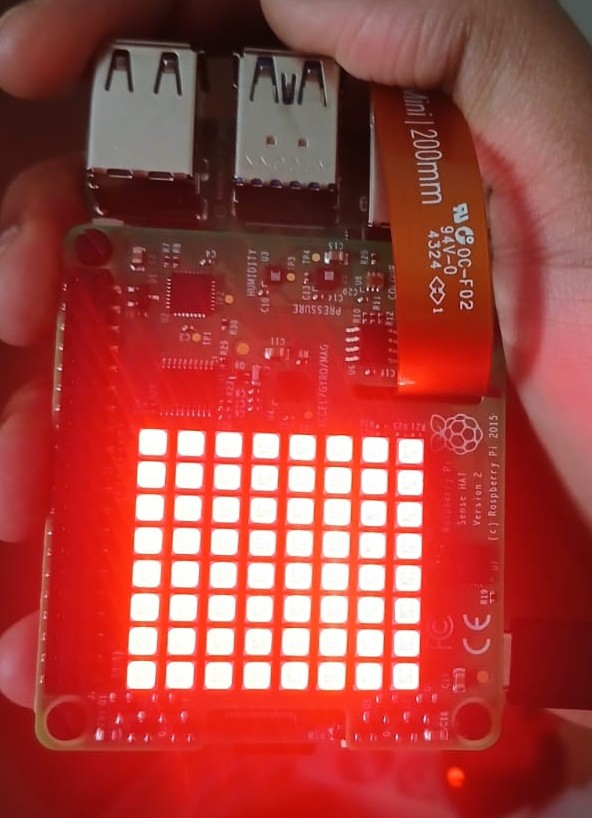
\includegraphics[width=3.5cm,height=3.5cm,keepaspectratio]{Red.jpg}
        \caption{(Red)}
        \label{fig:red}
    \end{subfigure}
    \hfill
    \begin{subfigure}[b]{0.23\textwidth}
        \centering
        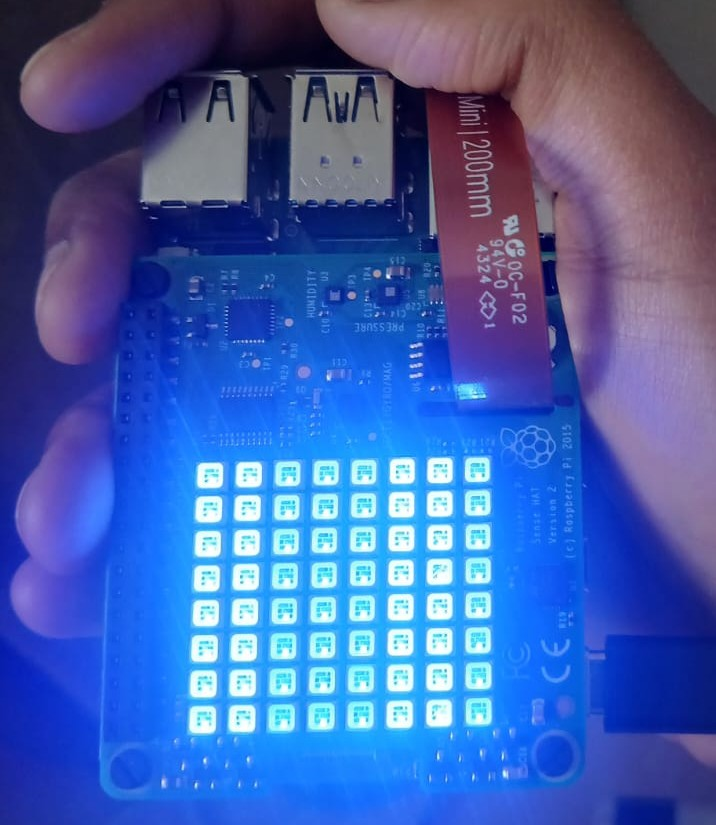
\includegraphics[width=3.5cm,height=3.5cm,keepaspectratio]{Blue.jpg}
        \caption{(Blue)}
        \label{fig:blue}
    \end{subfigure}
    \hfill
    \begin{subfigure}[b]{0.23\textwidth}
        \centering
        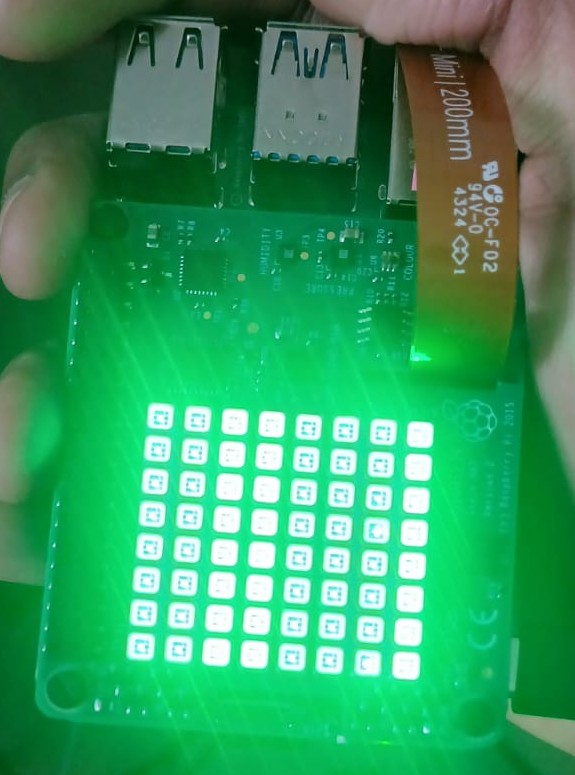
\includegraphics[width=3.5cm,height=3.5cm,keepaspectratio]{Green.jpg}
        \caption{Green}
        \label{fig:green}
    \end{subfigure}
    \hfill
    \begin{subfigure}[b]{0.23\textwidth}
        \centering
        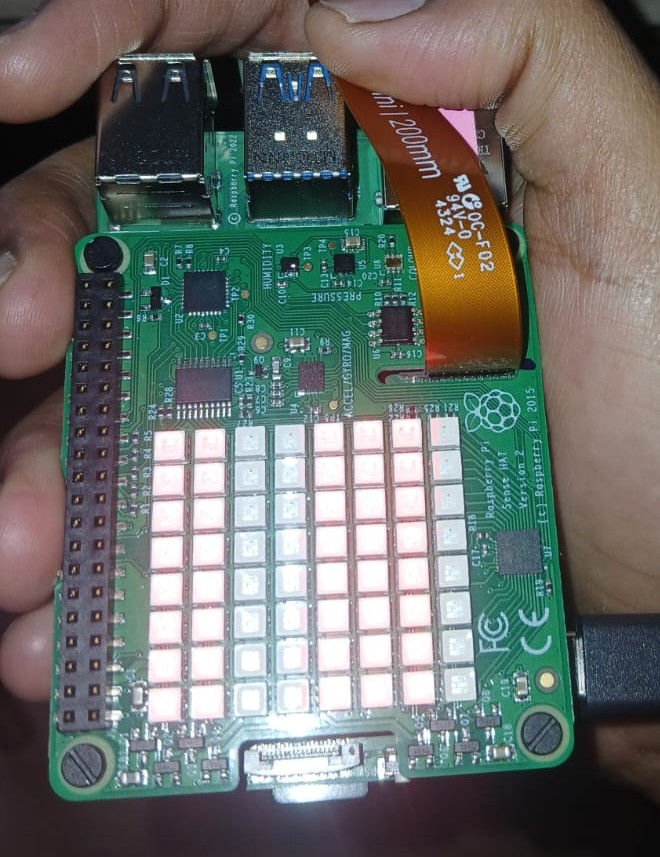
\includegraphics[width=3.5cm,height=3.5cm,keepaspectratio]{Colourless.jpg}
        \caption{Colourless}
        \label{fig:yellow}
    \end{subfigure}

    \caption{LED matrix output showing gesture recognition for four motion types, red for circular motion, green for shaking, blue for twist and colour does not change when motion does not changes.}
    \label{fig:all_gestures}
\end{figure}

\section{Challenges, Limitations, and Error Analysis}

\subsection{Challenges Faced}
\begin{itemize}
    \item Synchronizing real-time data capture and classification on Raspberry Pi.
    \item Differentiating similar motion patterns like shake and twist.
\end{itemize}

\subsection{Error Analysis}
\begin{itemize}
    \item The model occasionally misclassified the shake as twist.
    \item Errors caused by drifting IMU sensor and inconsistent user gesture speeds.
\end{itemize}

\subsection{Limitations of the Implementation}
\begin{itemize}
    \item Limited to four predefined gestures.
    \item The model does not generalize well to new users without retraining.
    \item Real-time inference performance is limited by the Raspberry Pi CPU capabilities.
\end{itemize}

\section{Discussion}
The results align with expectations, showing that simple feedforward neural networks can effectively classify motion data when provided with consistent samples. The use of TensorFlow Lite enables real-time inference on embedded hardware with limited resources. Future improvements could involve leveraging recurrent neural networks (e.g., LSTM) to better capture temporal dependencies in the IMU time series data.

\section{Conclusion}
This lab successfully demonstrated the end-to-end pipeline of collecting IMU sensor data, training a neural network model, converting it to TensorFlow Lite, and deploying it on a Raspberry Pi to perform real-time gesture recognition. The project highlights the practical application of machine learning techniques embedded in resource-constrained environments.

\section{References}
\begin{itemize}
    \item TensorFlow Documentation: \url{https://www.tensorflow.org}
    \item Sense HAT API: \url{https://pythonhosted.org/sense-hat/}
    \item Prof. Tobias Schaffer, Embedded Systems Lab05 Notes
\end{itemize}
\end{document}

\end{document}